\documentclass[12pt,a4paper,twoside]{article}

% ------------------------------------------------------------------ pacotes
\usepackage[T1]{fontenc}
\usepackage[utf8]{inputenc}
\usepackage[brazil]{babel}
\usepackage{lmodern}
\usepackage{microtype}
\usepackage[a4paper,margin=2.5cm]{geometry}
\usepackage{amsmath,amssymb,amsthm,bm}
\usepackage{graphicx}
\usepackage{booktabs,array,tabularx,multirow}
\usepackage{caption,subcaption}
\usepackage{xcolor}
\usepackage{tikz}
\usetikzlibrary{arrows.meta,angles,quotes,calc,patterns,babel}
\usepackage[output-decimal-marker={,}, group-separator={.}, range-phrase={ a }, list-final-separator={ e }, list-pair-separator={ e }, list-separator={; }]{siunitx}
\usepackage{enumitem}
\usepackage{csquotes}
\usepackage[style=abnt,backend=biber]{biblatex}
\addbibresource{referencias.bib}
\usepackage{fancyhdr}
\usepackage{setspace}
\usepackage{longtable}
\usepackage{indentfirst}
\setlength{\parindent}{1.5em}
\onehalfspacing
\pagestyle{fancy}
\fancyhf{}
\fancyhead[LE,RO]{Relatório Parcial}
\fancyhead[RE,LO]{PMR3220 - Projeto de Mecanismos}
\fancyfoot[LE,RO]{\thepage}
\fancyfoot[RE,LO]{\textit{\nouppercase{\leftmark}}}
\renewcommand{\sectionmark}[1]{\markboth{#1}{}}
\renewcommand{\headrulewidth}{0.4pt}
\renewcommand{\footrulewidth}{0.4pt}
\usepackage[hidelinks]{hyperref}
\usepackage[brazilian,capitalise,noabbrev]{cleveref}
\usepackage{listings}

\lstset{basicstyle=\ttfamily\footnotesize, breaklines=true, frame=single,
        literate={á}{{\'a}}1 {ã}{{\~a}}1 {é}{{\'e}}1 {ç}{{\c{c}}}1 {õ}{{\~o}}1 {í}{{\'i}}1 {ó}{{\'o}}1}

% gerado por scripts/parte1_parcial.py -- nao editar
\newcommand{\phiA}{0{,}0}
\newcommand{\phiB}{51{,}7}
\newcommand{\phiC}{97{,}2}
\newcommand{\phiD}{131{,}9}
\newcommand{\pernamin}{356}
\newcommand{\pernamax}{367}
\newcommand{\deslJ}{64}
\newcommand{\tabelaposes}{234 $\dagger$ & 15{,}4 & \ensuremath{-}11{,}7 & \ensuremath{-}59{,}4 & \ensuremath{-}70{,}8 & \ensuremath{-}413{,}8 & 359 \\
307 & 0{,}0 & 2{,}7 & \ensuremath{-}62{,}2 & 39{,}6 & \ensuremath{-}419{,}0 & 359 \\
390 & 51{,}7 & \ensuremath{-}29{,}9 & \ensuremath{-}53{,}6 & \ensuremath{-}293{,}2 & \ensuremath{-}309{,}4 & 367 \\
423 & 97{,}2 & \ensuremath{-}45{,}4 & \ensuremath{-}32{,}2 & \ensuremath{-}401{,}0 & \ensuremath{-}24{,}3 & 356 \\
456 & 131{,}9 & \ensuremath{-}46{,}2 & \ensuremath{-}20{,}3 & \ensuremath{-}338{,}0 & 191{,}7 & 361 \\
561 $\dagger$ & 155{,}1 & \ensuremath{-}59{,}1 & \ensuremath{-}5{,}1 & \ensuremath{-}235{,}4 & 291{,}2 & 345 \\}


\newcommand{\ve}[1]{\bm{#1}}
% --- notacao do metodo matricial (PMR3220) ---
\DeclareMathOperator{\sen}{sen}
\newcommand{\rv}[2]{{}^{#1}\mathbf{r}_{#2}}          % vetor posicao do ponto #2 na base #1
\newcommand{\rvd}[2]{{}^{#1}\dot{\mathbf{r}}_{#2}}
\newcommand{\rvdd}[2]{{}^{#1}\ddot{\mathbf{r}}_{#2}}
\newcommand{\vv}[2]{{}^{#1}\mathbf{v}_{#2}}
\newcommand{\Tm}[2]{{}^{#1}T_{#2}}                   % transformacao homogenea da base #2 para a base #1
\newcommand{\Tmd}[2]{{}^{#1}\dot T_{#2}}
\newcommand{\Tmdd}[2]{{}^{#1}\ddot T_{#2}}
\newcommand{\Rm}[2]{[{}^{#1}R_{#2}]}                 % matriz de rotacao
\newcommand{\Rot}[2]{\mathrm{Rot}(#1,\,#2)}
\newcommand{\hmg}[1]{\begin{bmatrix} #1 \\ 1 \end{bmatrix}}
\newcommand{\hoz}[1]{\begin{bmatrix} #1 \\ 0 \end{bmatrix}}
\newcommand{\Jm}[1]{[J_{#1}]}
\newcommand{\e}{\mathrm{e}}
\newcommand{\dd}{\,\mathrm{d}}
\newtheorem{hipotese}{Hipótese}
\captionsetup{font=small,labelsep=colon}
\numberwithin{equation}{section}

% ------------------------------------------------------------------ capa
\begin{document}
\begin{titlepage}
  \centering
  {\Large\bfseries ESCOLA POLITÉCNICA DA UNIVERSIDADE DE SÃO PAULO\par}
  \vspace{1.2cm}
  {\large\bfseries PMR3220 - Projeto de Mecanismos\par}
  \vspace{0.8cm}
  Prof. Dr. Ricardo Cury Ibrahim\par
  Prof. Dr. Tarcisio Antonio Hess Coelho\par
  \vspace{0.9cm}
  {\bfseries Grupo C\par}
  \vspace{0.5cm}
  \begin{spacing}{1.6}
  André Neme Benedetti - NUSP\par
  André Tsukassa Nishimoto - NUSP\par
  Felipe Wassmer Magina - NUSP\par
  Júlio Cesar de Andrade Oliveira - NUSP\par
  Lucas Sung Il Hong - NUSP\par
  Matheus Moreira de Sousa - NUSP\par
  Matheus Paixão de Sousa - NUSP\par
  Pedro Henrique Brasileiro de Jesus - NUSP\par
  \end{spacing}
  \vspace{0.7cm}
  {\LARGE Relatório Parcial\par}
  \vspace{0.3cm}
  {\bfseries Prótese e órtese de membro inferior\par}
  \vspace{0.8cm}
  
\includegraphics[width=4.2cm]{figuras/logo_poli_usp.png}\par
  \vfill
  {\large\bfseries São Paulo, 7 de outubro de 2026\par}
\end{titlepage}

\pagenumbering{roman}
\listoffigures
\clearpage
\listoftables
\clearpage
\tableofcontents
\clearpage
\pagenumbering{arabic}
\setcounter{page}{5}

\section{Introdução}

O movimento do membro inferior humano resulta da interação entre diferentes segmentos
e articulações, sendo o joelho particularmente importante para a mobilidade entre a
coxa e a perna. Entretanto, seu movimento relativo não pode ser rigorosamente
representado por uma simples junta de revolução: no plano sagital, os côndilos
femorais rolam e deslizam sobre o platô tibial, de modo que o centro instantâneo de
rotação (CIR) descreve uma trajetória -- a \emph{centroide} -- em vez de permanecer fixo
\cite{menschik1974,oconnor1989,dathe2016}. Desde \textcite{menschik1974}, essa cinemática
é modelada por um quadrilátero articulado cruzado, formado pelas fibras isométricas
dos ligamentos cruzados anterior (LCA) e posterior (LCP) e pelos segmentos ósseos que
unem suas inserções \cite{oconnor1989,zavatsky1992}.

Nesse contexto, o projeto de próteses e órteses constitui uma aplicação relevante da
teoria de mecanismos, permitindo reproduzir ou auxiliar movimentos do membro inferior
em situações de amputação ou de comprometimento da capacidade motora. Este relatório
parcial trata da primeira etapa do trabalho: o projeto de uma prótese de joelho e
perna capaz de reproduzir o movimento relativo entre a coxa e o conjunto perna--pé por
meio de um quadrilátero articulado plano (\cref{fig:enunciado}). São apresentados a
fundamentação do modelo, a definição da geometria, a aquisição experimental do
movimento em um integrante do grupo e o processamento dos dados que servirá de base
para a síntese dimensional do mecanismo.

\begin{figure}[htbp]
  \centering
  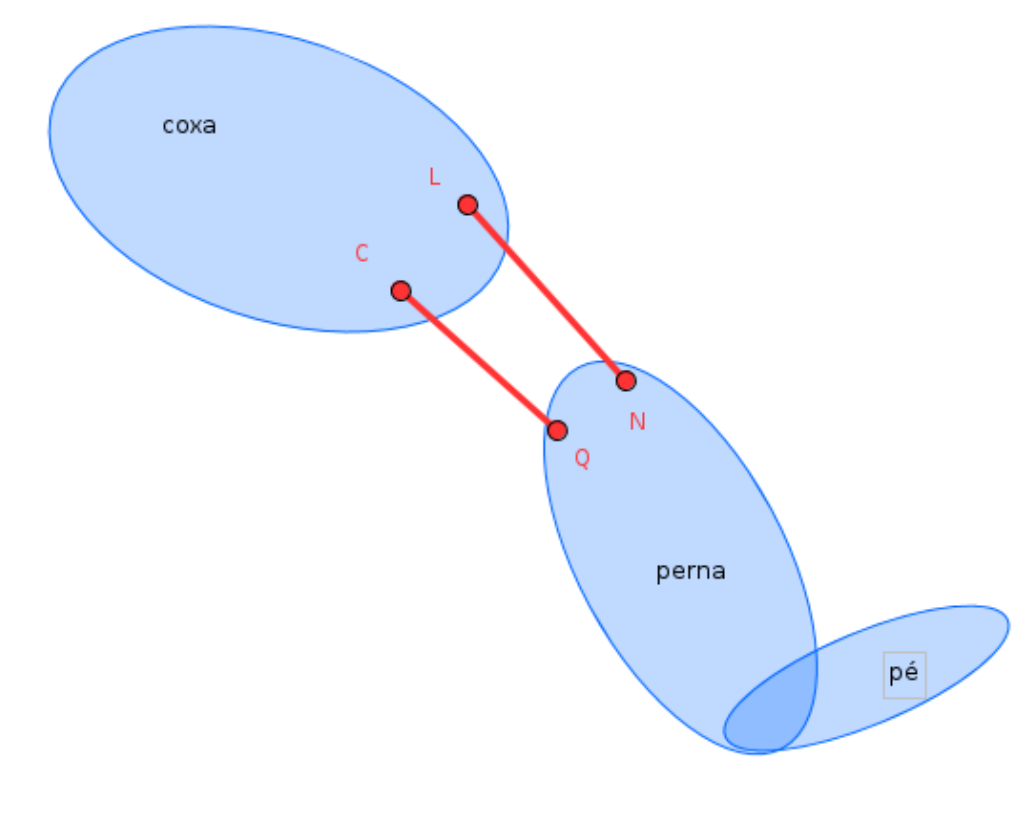
\includegraphics[width=0.42\textwidth]{figuras/enunciado_fig1.png}
  \caption{Diagrama cinemático do enunciado: pivôs $C$ e $L$ na coxa e $Q$ e $N$ na perna.}
  \label{fig:enunciado}
\end{figure}

\section{Objetivos}

\begin{itemize}
  \item Desenvolver a síntese dimensional de um mecanismo quadrilátero articulado,
  capaz de reproduzir de forma aproximada o movimento relativo entre a coxa e o
  conjunto perna--pé de uma prótese de membro inferior.
  \item Determinar as dimensões e as posições das articulações do mecanismo, utilizando
  como referência as posições do membro inferior obtidas experimentalmente.
  \item Realizar a análise cinemática de uma órtese para membro inferior, determinando
  as posições, velocidades e acelerações angulares dos segmentos ao longo de um ciclo
  de movimento.
  \item Realizar a análise dinâmica do sistema, determinando os torques necessários nos
  atuadores do joelho e da articulação entre a coxa e o tronco para a execução do
  movimento considerado.
\end{itemize}

Neste relatório parcial são desenvolvidas as etapas preparatórias do primeiro e do
segundo objetivos: a formulação do modelo do quadrilátero e a obtenção, a partir das
medições, do movimento relativo entre a coxa e a perna.

\section{Fundamentação teórica}\label{cap:teoria1}

\subsection{Notação}\label{sec:notacao}

A modelagem cinemática segue o \emph{método matricial} adotado na disciplina, baseado em
transformações homogêneas. A cada elo $i$ associa-se uma base (sistema de referência)
$O_iX_iY_iZ_i$, de versores $\mathbf i_i$, $\mathbf j_i$, $\mathbf k_i$; a base $0$ é fixa. As
convenções são:
\begin{itemize}
  \item $\rv{A}{P}$: vetor posição do ponto $P$ escrito na base $A$ (o sobrescrito à esquerda
  indica a base);
  \item $\Rm{A}{B} = [\,{}^{A}\mathbf i_B,\ {}^{A}\mathbf j_B,\ {}^{A}\mathbf k_B\,]$: matriz de rotação
  cujas colunas são os versores da base $B$ escritos na base $A$, com
  $\Rm{B}{A} = \Rm{A}{B}^{-1} = \Rm{A}{B}^{\mathsf T}$;
  \item rotação simples de ângulo $\gamma$ em torno do eixo $z_B$ (movimento plano):
  \begin{equation}
    \Rm{A}{B} = \Rot{\gamma}{z_B} =
    \begin{bmatrix} \cos\gamma & -\sen\gamma & 0\\ \sen\gamma & \cos\gamma & 0\\ 0 & 0 & 1 \end{bmatrix},
    \qquad
    \begin{aligned}
      \mathbf i_B &= \cos\gamma\,\mathbf i_A + \sen\gamma\,\mathbf j_A,\\
      \mathbf j_B &= -\sen\gamma\,\mathbf i_A + \cos\gamma\,\mathbf j_A,\\
      \mathbf k_B &= \mathbf k_A;
    \end{aligned}
  \end{equation}
  no plano, usa-se apenas o bloco $2\times2$ superior;
  \item mudança de base de um ponto: $\rv{A}{P} = \Rm{A}{B}\,\rv{B}{P} + \rv{A}{O_B}$, ou, na forma
  homogênea,
  \begin{equation}
    \hmg{\rv{A}{P}} = \Tm{A}{B}\hmg{\rv{B}{P}},
    \qquad
    \Tm{A}{B} = \left[\begin{array}{c|c} \Rm{A}{B} & \rv{A}{O_B} \\ \hline \mathbf 0 & 1 \end{array}\right],
    \label{eq:homogenea}
  \end{equation}
  e, para uma cadeia de elos, $\Tm{0}{n} = \Tm{0}{1}\,\Tm{1}{2}\cdots\Tm{n-1}{n}$;
  \item abreviações: $c_i = \cos\theta_i$, $s_i = \sen\theta_i$, $c_{ij} = \cos(\theta_i+\theta_j)$,
  $s_{ij} = \sen(\theta_i+\theta_j)$; o ângulo $\theta_i$ da junta $i$ é medido do eixo $X_{i-1}$ ao
  eixo $X_i$ (ângulo \emph{relativo}), positivo no sentido anti-horário;
  \item produto vetorial na forma matricial: $\mathbf a \times \mathbf b = \tilde{\mathbf a}\,\mathbf b$, com
  $\tilde{\mathbf a} = \begin{bmatrix} 0 & -a_z & a_y\\ a_z & 0 & -a_x\\ -a_y & a_x & 0\end{bmatrix}$.
\end{itemize}

\subsection{Quadrilátero articulado e o joelho policêntrico}

Um quadrilátero articulado plano possui quatro elos ligados por quatro juntas de
revolução e, pelo critério de Grübler, um grau de liberdade:
\begin{equation}
  M = 3(n-1) - 2j_1 - j_2 = 3(4-1) - 2\cdot 4 - 0 = 1 .
\end{equation}
No joelho protético (\cref{fig:enunciado}) o elo fixo é a coxa (pivôs $C$ e $L$),
as manivelas/balancins são $CQ$ e $LN$, e o \emph{acoplador} é a perna (pivôs $Q$ e $N$),
ao qual se fixa rigidamente o pé. Como o acoplador executa um movimento plano geral,
seu CIR relativo à coxa -- o polo $I_{13}$ -- é, pelo teorema de Aronhold--Kennedy, a
intersecção das retas $CQ$ e $LN$ e se desloca à medida que o joelho flexiona, tal como
no joelho natural \cite{norton2010,radcliffe1994}. Joelhos protéticos de quatro barras
exploram essa propriedade: com o CIR alto e posterior na extensão, obtém-se
estabilidade voluntária na fase de apoio; com o CIR migrando na flexão, obtém-se
encurtamento aparente da perna na fase de balanço \cite{radcliffe1994}.

A condição de Grashof classifica o tipo de movimento possível. Sendo $s$ e $l$ os
comprimentos do menor e do maior elo e $p$, $q$ os demais,
\begin{equation}
  s + l \le p + q \quad\Longrightarrow\quad \text{pelo menos um elo dá voltas completas.}
  \label{eq:grashof}
\end{equation}
Na prótese, a flexão útil está limitada a cerca de \SI{120}{\degree}; logo, um mecanismo
não Grashof (triplo balancim) é aceitável, desde que nenhuma configuração de ponto
morto ocorra dentro dessa faixa. A qualidade da transmissão de forças é avaliada pelo
ângulo de transmissão $\mu$ -- ângulo agudo entre o acoplador e o balancim de saída --,
recomendando-se $\mu \ge \SI{30}{\degree}$ \cite{norton2010}.

\subsection{Bases e análise de posição do quadrilátero (cadeia fechada)}\label{sec:cadeia_fechada}

A \cref{fig:quadrilatero} mostra as bases adotadas, seguindo a convenção da
\cref{sec:notacao}. A base $0$ (fixa) está presa à coxa, com origem no centro do joelho em
extensão, $X_0$ para a frente (anterior) e $Y_0$ para cima (proximal). As bases $1$, $2$ e $3$
estão presas, respectivamente, ao elo $CQ$ (origem em $C$, $X_1$ ao longo de $CQ$), ao
acoplador (origem em $Q$, $X_2$ ao longo de $QN$) e ao elo $LN$ (origem em $L$, $X_3$ ao longo
de $LN$). A base $4$ também está presa à perna, com origem no ponto de referência do
joelho e $Y_4$ ao longo do eixo da perna (é a base em que se fazem as medições). Os
comprimentos são $\ell_0 = \overline{CL}$, $\ell_1 = \overline{CQ}$, $\ell_2 = \overline{QN}$ e
$\ell_3 = \overline{LN}$.

\begin{figure}[htbp]
  \centering
  \begin{tikzpicture}[scale=1.35, >=Stealth]
    \coordinate (C) at (0,0);
    \coordinate (L) at (3,0.6);
    \coordinate (Q) at ({1.6*cos(115)},{1.6*sin(115)});
    \coordinate (N) at ($(L)+({2.4*cos(128)},{2.4*sin(128)})$);
    \draw[thick] (C) -- node[left, pos=0.6] {$\ell_1$} (Q) -- node[above left, pos=0.6] {$\ell_2$} (N) -- node[right] {$\ell_3$} (L);
    \draw[thick,dashed,gray] (C) -- node[below] {$\ell_0$} (L);
    \foreach \p in {C,Q,N,L} \draw[fill=white] (\p) circle (0.06);
    \node[below left] at (C) {$C$}; \node[below right] at (L) {$L$};
    \node[left] at (Q) {$Q$}; \node[above right] at (N) {$N$};
    % base 0
    \draw[->,thick] (-1.2,-0.8) -- (-0.4,-0.8) node[below] {$X_0$};
    \draw[->,thick] (-1.2,-0.8) -- (-1.2,0) node[left] {$Y_0$};
    % base 1
    \draw[->,teal] (C) -- ($(C)!0.45!(Q)$) node[right=2pt] {$X_1$};
    \draw[dashed,blue] (C) -- (1,0) coordinate (Ce);
    \pic[draw,->,blue,"$\theta_1$",angle radius=0.5cm,angle eccentricity=1.45] {angle=Ce--C--Q};
    % base 2
    \coordinate (Qe) at ($(Q)!-0.5!(C)$);
    \draw[dashed,blue] (Q) -- (Qe);
    \draw[->,teal] (Q) -- ($(Q)!0.3!(N)$) node[below] {$X_2$};
    \pic[draw,->,blue,"$\theta_2$",angle radius=0.45cm,angle eccentricity=1.5] {angle=N--Q--Qe};
    % base 3
    \draw[dashed,blue] (L) -- ($(L)+(0.8,0.16)$) coordinate (Le);
    \draw[->,teal] (L) -- ($(L)!0.25!(N)$) node[left] {$X_3$};
    \pic[draw,->,blue,"$\theta_3$",angle radius=0.45cm,angle eccentricity=1.5] {angle=Le--L--N};
    \node[gray] at (0.4,2.8) {perna (acoplador)};
    \node[gray] at (1.5,-0.6) {coxa (elo fixo 0)};
  \end{tikzpicture}
  \caption{Quadrilátero articulado do joelho: bases, ângulos e comprimentos (a base $1$ e a
  base $3$ têm os ângulos medidos a partir de $X_0$; $\theta_2$ é medido a partir de $X_1$).}
  \label{fig:quadrilatero}
\end{figure}

As transformações homogêneas \eqref{eq:homogenea} de cada elo são
\begin{equation}
  \Tm{0}{1} = \left[\begin{array}{cc|c} c_1 & -s_1 & {}^0x_C\\ s_1 & c_1 & {}^0y_C\\ \hline 0 & 0 & 1\end{array}\right],\quad
  \Tm{1}{2} = \left[\begin{array}{cc|c} c_2 & -s_2 & \ell_1\\ s_2 & c_2 & 0\\ \hline 0 & 0 & 1\end{array}\right],\quad
  \Tm{0}{3} = \left[\begin{array}{cc|c} c_3 & -s_3 & {}^0x_L\\ s_3 & c_3 & {}^0y_L\\ \hline 0 & 0 & 1\end{array}\right],
\end{equation}
com $\rv{2}{N} = [\ell_2\ \ 0]^{\mathsf T}$ e $\rv{3}{N} = [\ell_3\ \ 0]^{\mathsf T}$. O ponto $N$ pertence
simultaneamente ao ramo $0\text{--}1\text{--}2$ e ao ramo $0\text{--}3$ da cadeia. Pelo ramo
$0\text{--}1\text{--}2$, multiplica-se primeiro o ponto pela matriz mais à direita:
\begin{equation*}
  \Tm{1}{2}\hmg{\rv{2}{N}} = \begin{bmatrix} \ell_2 c_2 + \ell_1 \\ \ell_2 s_2 \\ 1\end{bmatrix},
  \qquad
  \Tm{0}{1}\begin{bmatrix} \ell_2 c_2 + \ell_1 \\ \ell_2 s_2 \\ 1\end{bmatrix}
  = \begin{bmatrix} {}^0x_C + \ell_1 c_1 + \ell_2(c_1c_2 - s_1s_2) \\ {}^0y_C + \ell_1 s_1 + \ell_2(s_1c_2 + c_1s_2) \\ 1\end{bmatrix},
\end{equation*}
e as identidades $c_1c_2 - s_1s_2 = c_{12}$ e $s_1c_2 + c_1s_2 = s_{12}$ simplificam o resultado.
Igualando ao ramo $0\text{--}3$, obtém-se a \emph{equação de fechamento}
\begin{equation}
  \hmg{\rv{0}{N}} = \Tm{0}{1}\,\Tm{1}{2}\hmg{\rv{2}{N}} = \Tm{0}{3}\hmg{\rv{3}{N}}
  \;\Longrightarrow\;
  \begin{bmatrix} {}^0x_C + \ell_1 c_1 + \ell_2 c_{12} \\ {}^0y_C + \ell_1 s_1 + \ell_2 s_{12} \\ 1 \end{bmatrix}
  = \begin{bmatrix} {}^0x_L + \ell_3 c_3 \\ {}^0y_L + \ell_3 s_3 \\ 1 \end{bmatrix}.
  \label{eq:fechamento}
\end{equation}
Na prótese, a variável de entrada é a orientação da perna, $\psi = \theta_1 + \theta_2$
(ângulo de $X_2$ em relação a $X_0$), e as incógnitas são $\mathbf q = [\theta_1\ \ \theta_3]^{\mathsf T}$.
Passando todos os termos de \eqref{eq:fechamento} para um lado, com $c_{12} = \cos\psi$ e
$s_{12} = \sen\psi$ conhecidos,
\begin{equation*}
  \mathbf f(\mathbf q) =
  \begin{bmatrix} {}^0x_C + \ell_1 c_1 + \ell_2\cos\psi - {}^0x_L - \ell_3 c_3 \\
                  {}^0y_C + \ell_1 s_1 + \ell_2\sen\psi - {}^0y_L - \ell_3 s_3 \end{bmatrix} = \mathbf 0 ,
\end{equation*}
cujas derivadas parciais em relação a $\theta_1$ e $\theta_3$ formam a matriz jacobiana. A
solução é obtida pelo método de Newton--Raphson,
\begin{equation}
  \mathbf q^{(i+1)} = \mathbf q^{(i)} - [J]^{-1}\,\mathbf f\big(\mathbf q^{(i)}\big),
  \qquad
  [J] = \frac{\partial\mathbf f}{\partial\mathbf q} =
  \begin{bmatrix} -\ell_1 s_1 & \ell_3 s_3 \\ \ell_1 c_1 & -\ell_3 c_3 \end{bmatrix},
  \label{eq:newton}
\end{equation}
partindo da solução do passo anterior, o que mantém o mecanismo no mesmo ramo de
montagem. Como $\det[J] = \ell_1\ell_3\,\sen(\theta_1 - \theta_3)$, a matriz é singular quando
$CQ \parallel LN$ (polo no infinito). Uma vez conhecidos $\theta_1$ e $\theta_3$, o polo
$I_{13}$ (CIR da perna em relação à coxa) é a intersecção dos eixos $X_1$ e $X_3$,
\begin{equation}
  \rv{0}{I} = \rv{0}{C} + \lambda\begin{bmatrix} c_1\\ s_1\end{bmatrix} = \rv{0}{L} + \kappa\begin{bmatrix} c_3\\ s_3\end{bmatrix},
\end{equation}
e o ângulo de transmissão é o ângulo agudo entre $X_2$ e $X_3$, $\mu = |\psi - \theta_3|$
(reduzido a $[0, \SI{90}{\degree}]$).

\section{Metodologia}\label{cap:metodos1}

\subsection{Definição da geometria do mecanismo}

Inicialmente, foi definida uma representação geométrica simplificada do membro
inferior humano, buscando preservar as principais características cinemáticas do
movimento da coxa, da perna e do pé. A coxa, a perna e o pé foram considerados como
elementos rígidos, representados pelas geometrias correspondentes às regiões do membro
inferior. Para representar o movimento relativo entre a coxa e a perna na região do
joelho, foi adotado um mecanismo quadrilátero articulado. A configuração adotada e a
identificação dos pontos utilizados no modelo são apresentadas na \cref{fig:geometria}.

\begin{figure}[htbp]
  \centering
  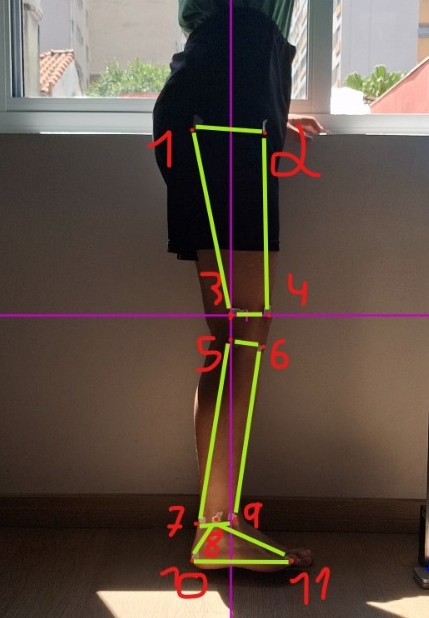
\includegraphics[width=0.36\textwidth]{figuras/rasc_p6_0.jpeg}
  \caption{Geometria adotada para a representação do membro inferior.}
  \label{fig:geometria}
\end{figure}

Na representação adotada, os pontos 1 e 2 estão localizados na região do quadril,
enquanto os pontos 3 e 4 estão posicionados na extremidade inferior da coxa, próxima à
região do joelho. Para a perna, os pontos 5 e 6 estão localizados imediatamente abaixo
do joelho, enquanto os pontos 7 e 9 estão posicionados aproximadamente na região do
tornozelo. O ponto 8 está localizado entre os pontos 7 e 9, contribuindo para a
representação da conexão entre a perna e o pé. Por fim, os pontos 10 e 11 correspondem
às extremidades inferiores da representação do pé.

A escolha de um mecanismo quadrilátero articulado para representar o movimento do
joelho está relacionada à necessidade de reproduzir adequadamente o movimento relativo
observado entre a coxa e a perna. Uma representação mais simples, na qual a coxa e a
perna fossem consideradas elementos rígidos conectados diretamente por uma única junta
de revolução, permitiria descrever apenas uma rotação da perna em torno de um centro
fixo. Nesse caso, os pontos pertencentes à perna descreveriam trajetórias circulares em
relação à coxa, o que constitui uma aproximação limitada do movimento do joelho.

O emprego de um quadrilátero articulado permite obter o movimento relativo entre a
coxa e a perna a partir da combinação das rotações de seus diferentes elos. Dessa
forma, o centro instantâneo do movimento relativo entre os segmentos (o polo $I_{13}$ da
\cref{sec:cadeia_fechada}) pode variar durante a movimentação, permitindo reproduzir
trajetórias mais complexas do que aquelas obtidas por uma única junta de revolução.
Essa característica é particularmente relevante para o problema proposto, uma vez que
o movimento relativo entre a coxa e a perna não pode ser rigorosamente representado
apenas por uma junta de rotação.

A representação do pé por meio de uma geometria triangular foi adotada de maneira
análoga, buscando preservar sua extensão e sua orientação em relação à perna. Uma
representação por um único elemento rígido poderia descrever apenas a distância entre
dois pontos, sem representar simultaneamente diferentes pontos de referência
associados ao pé. A geometria triangular fornece, portanto, uma representação rígida
simplificada da região, possibilitando acompanhar sua posição e orientação durante o
movimento.

Embora os pontos utilizados na aquisição experimental tenham sido definidos próximos
aos vértices das regiões utilizadas na representação geométrica, a localização das
articulações do mecanismo não está necessariamente restrita a esses pontos
experimentais. Articulações localizadas no interior das regiões correspondentes à coxa
e à perna também podem ser consideradas durante a síntese, desde que sejam compatíveis
com a geometria e com o movimento desejado.

\subsection{Aquisição experimental do movimento}\label{sec:aquisicao}

Após a definição da geometria, foram realizadas medições experimentais com o objetivo
de obter as posições dos pontos de interesse ao longo do movimento do membro inferior.
Para isso, um integrante do grupo realizou o movimento com a própria perna, e foi
registrada uma sequência de vídeo com o membro observado lateralmente.

Foram consideradas três configurações principais para caracterizar o movimento. A
configuração inicial corresponde à posição em pé, na qual a coxa, a perna e o pé se
encontram aproximadamente alinhados. A configuração intermediária corresponde a uma
flexão da perna de aproximadamente \SI{90}{\degree} em relação à coxa, mantendo-se a
posição da coxa. Por fim, a configuração final corresponde à condição de maior flexão
observada durante o experimento, na qual a perna se aproxima da coxa. A sequência de
configurações observada durante o movimento é apresentada na \cref{fig:sequencia}.

\begin{figure}[htbp]
  \centering
  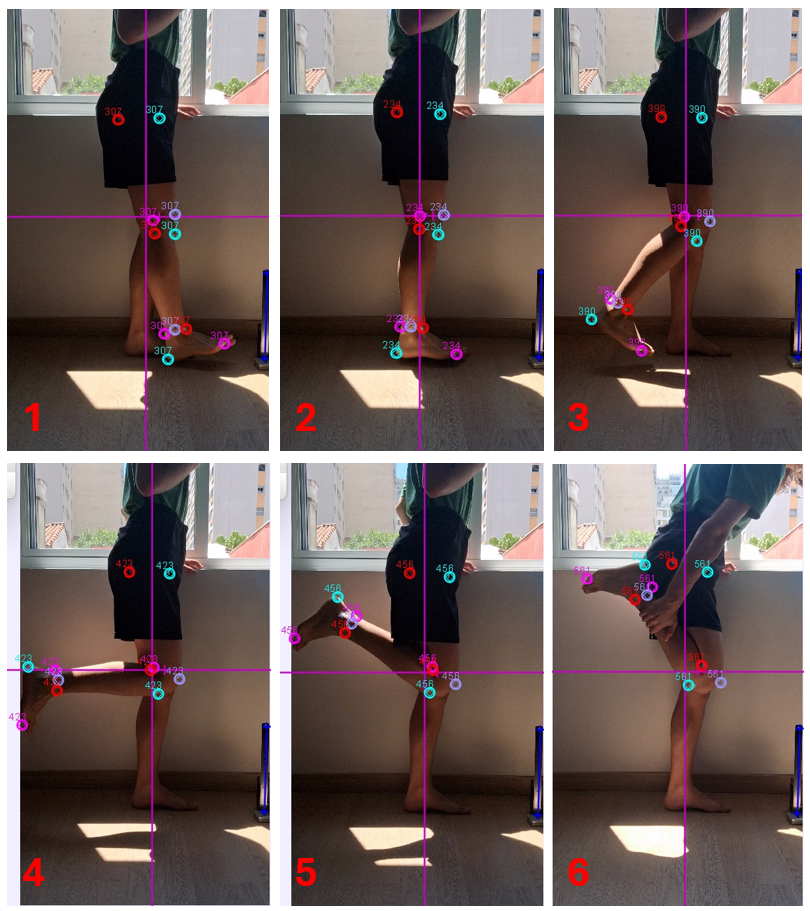
\includegraphics[width=0.62\textwidth]{figuras/rasc_p7_0.png}
  \caption{Sequência de configurações do membro inferior durante o movimento experimental.}
  \label{fig:sequencia}
\end{figure}

Para o processamento do vídeo foi empregado o software \emph{Tracker} \cite{tracker},
que permite acompanhar a posição de pontos específicos ao longo dos diferentes
\emph{frames} de uma gravação. Foram definidos pontos de referência próximos aos
vértices das regiões utilizadas na representação geométrica da coxa, da perna e do pé.
Esses pontos foram identificados e acompanhados individualmente ao longo do movimento,
permitindo obter suas coordenadas no plano da imagem em função do tempo. A numeração
dos pontos utilizada no rastreamento corresponde à geometria apresentada anteriormente
(\cref{fig:geometria}).

\begin{figure}[htbp]
  \centering
  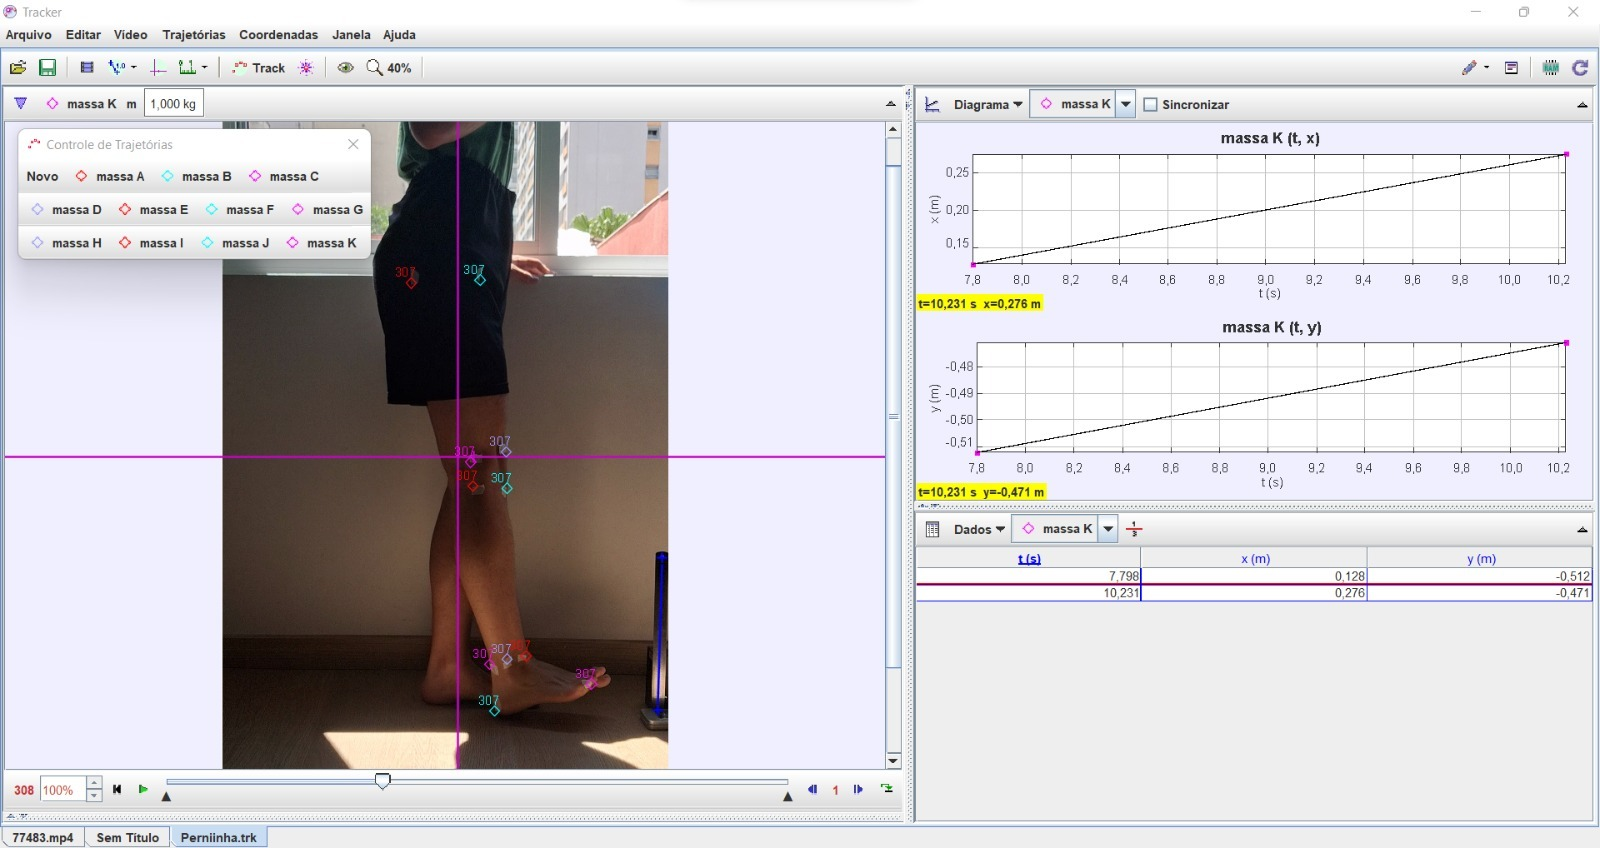
\includegraphics[width=\textwidth]{figuras/rasc_p8_0.jpeg}
  \caption{Rastreamento dos pontos do membro inferior e obtenção das posições no software \emph{Tracker}.}
  \label{fig:tracker}
\end{figure}

A partir do rastreamento, o \emph{Tracker} forneceu as coordenadas $x$ e $y$ dos pontos
acompanhados para os diferentes instantes analisados. Os valores obtidos correspondem,
portanto, às posições dos pontos no plano da imagem (base $im$, com a escala calibrada
em metros), e não diretamente aos comprimentos dos elos do mecanismo. O software também
permitiu visualizar graficamente a evolução temporal dessas coordenadas.

A planilha de dados obtida a partir do rastreamento contém as coordenadas dos onze
pontos para os \emph{frames} 234, 307, 390, 423, 456 e 561 (\cref{tab:tracker}, na
\cref{sec:anexos}). Para a análise do movimento, foram selecionados os \emph{frames}
307, 390, 423 e 456. O \emph{frame} 234 foi utilizado como referência durante a
identificação e numeração dos pontos, enquanto o \emph{frame} 561 foi desconsiderado,
pois corresponde a uma etapa do movimento em que houve auxílio manual para conduzir a
perna.

\subsection{Processamento dos dados}\label{sec:processamento}

As coordenadas do \emph{Tracker} estão na base da imagem. O que interessa ao quadrilátero
do joelho é apenas o movimento \emph{relativo} entre a coxa e a perna; por isso, o
movimento angular do quadril (a rotação da coxa em relação ao tronco, que também ocorre
levemente durante o experimento) foi desconsiderado, e a coxa foi tratada como o elo
fixo do mecanismo. Os dados foram processados em dois passos.

\paragraph{1º passo -- base da coxa em cada quadro.} A base $0$ tem origem no ponto médio
dos marcadores 3 e 4 (extremidade distal da coxa, junto ao joelho) e eixos paralelos aos
da imagem: $X_0$ horizontal, para a frente, e $Y_0$ vertical, para cima. Como a rotação do
quadril é desconsiderada, $\Rm{im}{0} = \Rot{0}{z_0} = I$, e a base da coxa apenas
acompanha a translação da região do joelho entre os quadros:
\begin{equation}
  \Tm{im}{0} = \left[\begin{array}{c|c} I & \tfrac12\big(\rv{im}{3} + \rv{im}{4}\big) \\ \hline \mathbf 0 & 1 \end{array}\right],
  \qquad
  \rv{0}{k} = \rv{im}{k} - \tfrac12\big(\rv{im}{3} + \rv{im}{4}\big).
\end{equation}
Os marcadores 1 e 2 (quadril) não entram no processamento.

\paragraph{2º passo -- orientação da perna e flexão do joelho.} A perna é representada pelo
segmento que vai do ponto $J$, médio dos marcadores 5 e 6 (logo abaixo do joelho), ao
ponto $P$, marcador 8 (conexão perna--pé). Na base da coxa, sua orientação é
\begin{equation}
  \beta_j = \operatorname{atan2}\big({}^0y_P - {}^0y_J,\ {}^0x_P - {}^0x_J\big),
\end{equation}
e a flexão do joelho no quadro $j$ é medida em relação ao quadro 307 (membro estendido):
\begin{equation}
  \varphi_j = \beta_{307} - \beta_j \pmod{\SI{360}{\degree}} .
\end{equation}

\begin{table}[htbp]
  \centering
  \caption{Posição da perna na base $0$ (coxa) obtida das medições (mm): ponto $J$ (abaixo
  do joelho), ponto $P$ (tornozelo) e comprimento $\overline{JP}$. $\dagger$: quadro não
  utilizado na análise.}
  \label{tab:poses}
  \begin{tabular}{lrrrrrr}
    \toprule
    Quadro & $\varphi$ (\si{\degree}) & ${}^0x_{J}$ & ${}^0y_{J}$ & ${}^0x_{P}$ & ${}^0y_{P}$ & $\overline{JP}$ \\
    \midrule
    \tabelaposes
    \bottomrule
  \end{tabular}
\end{table}

\begin{figure}[htbp]
  \centering
  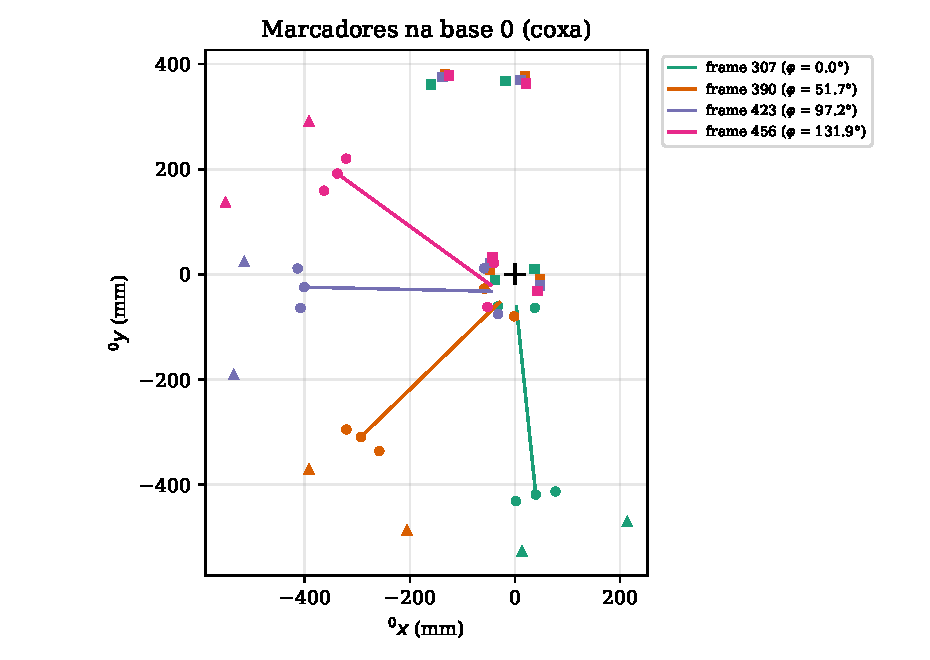
\includegraphics[width=0.85\textwidth]{figuras/parcial_medicoes.pdf}
  \caption{Marcadores dos quadros selecionados escritos na base da coxa, com origem entre
  os pontos 3 e 4 ($\square$: coxa, $\circ$: perna, $\triangle$: pé; linha: segmento $JP$).}
  \label{fig:medicoes}
\end{figure}

Os quadros selecionados correspondem a flexões de \phiA, \phiB, \phiC{} e
\phiD\si{\degree} (\cref{tab:poses,fig:medicoes}), próximas das configurações inicial
(\SI{0}{\degree}), intermediárias (cerca de \SI{45}{\degree} e \SI{90}{\degree}) e de
máxima flexão. O comprimento do segmento $JP$ varia apenas entre \pernamin{} e
\pernamax~mm, o que confirma a coerência da marcação ao longo do movimento (as
diferenças decorrem dos artefatos de pele e da marcação manual). Observa-se ainda que
o ponto $J$, logo abaixo do joelho, desloca-se cerca de \deslJ~mm em relação à coxa entre
a extensão e a flexão máxima: a perna não gira em torno de um ponto fixo, o que
confirma que uma junta de revolução simples não reproduz o movimento e motiva o uso do
quadrilátero articulado.

\section{Conclusões}

Nesta etapa, foram definidos a geometria de representação do membro inferior e o
modelo do joelho protético como quadrilátero articulado, formulado pelo método
matricial. O movimento do membro de um integrante do grupo foi filmado e rastreado no
\emph{Tracker}, e os dados foram escritos na base da coxa, desconsiderando o movimento
angular do quadril. Os quatro quadros selecionados cobrem flexões do joelho de
\phiA{} a \phiD\si{\degree}, e o deslocamento de cerca de \deslJ~mm da região proximal
da perna em relação à coxa confirma que o movimento relativo não é uma rotação pura.

As próximas etapas são: a síntese dimensional do quadrilátero a partir das posições
medidas, a construção da maquete e a análise cinemática e dinâmica da órtese.

\section{Materiais e anexos}\label{sec:anexos}

Os arquivos utilizados na aquisição e no tratamento dos dados experimentais são
disponibilizados juntamente com o relatório, incluindo o arquivo do projeto utilizado
no software \emph{Tracker}, a planilha com as coordenadas obtidas durante o rastreamento
e o programa em Python usado no processamento (\texttt{scripts/parte1\_parcial.py}).

\subsection{Dados experimentais obtidos pelo \emph{Tracker}}

A tabela a seguir apresenta as coordenadas cartesianas dos onze pontos rastreados para os
\emph{frames} registrados durante o experimento. Os valores correspondem diretamente aos
dados obtidos no arquivo de saída utilizado para a organização dos resultados
experimentais.

{\small
\begin{longtable}{cc rr}
  \caption{Coordenadas dos pontos obtidas pelo \emph{Tracker}.}\label{tab:tracker}\\
  \toprule
  Frame & Ponto & $x$ (m) & $y$ (m) \\
  \midrule
  \endfirsthead
  \toprule
  Frame & Ponto & $x$ (m) & $y$ (m) \\
  \midrule
  \endhead
  \midrule
  \multicolumn{4}{r}{Continua na próxima página}\\
  \endfoot
  \bottomrule
  \endlastfoot
    234 & 1 & \ensuremath{-}0.078146 & 0.386447 \\
    234 & 2 & 0.069715 & 0.381067 \\
    234 & 3 & 0.000380 & 0.000035 \\
    234 & 4 & 0.084056 & 0.004970 \\
    234 & 5 & \ensuremath{-}0.003477 & \ensuremath{-}0.046264 \\
    234 & 6 & 0.064449 & \ensuremath{-}0.067460 \\
    234 & 7 & \ensuremath{-}0.067107 & \ensuremath{-}0.412356 \\
    234 & 8 & \ensuremath{-}0.028615 & \ensuremath{-}0.411334 \\
    234 & 9 & 0.010899 & \ensuremath{-}0.415762 \\
    234 & 10 & \ensuremath{-}0.081579 & \ensuremath{-}0.508887 \\
    234 & 11 & 0.128059 & \ensuremath{-}0.512169 \\
    307 & 1 & \ensuremath{-}0.096598 & 0.361130 \\
    307 & 2 & 0.045186 & 0.368099 \\
    307 & 3 & 0.025422 & \ensuremath{-}0.010538 \\
    307 & 4 & 0.100385 & 0.010706 \\
    307 & 5 & 0.030582 & \ensuremath{-}0.060615 \\
    307 & 6 & 0.100689 & \ensuremath{-}0.063650 \\
    307 & 7 & 0.064449 & \ensuremath{-}0.431417 \\
    307 & 8 & 0.102506 & \ensuremath{-}0.418892 \\
    307 & 9 & 0.140082 & \ensuremath{-}0.413111 \\
    307 & 10 & 0.076024 & \ensuremath{-}0.527587 \\
    307 & 11 & 0.276455 & \ensuremath{-}0.470734 \\
    390 & 1 & \ensuremath{-}0.092092 & 0.369497 \\
    390 & 2 & 0.059443 & 0.364994 \\
    390 & 3 & \ensuremath{-}0.006151 & \ensuremath{-}0.003193 \\
    390 & 4 & 0.087942 & \ensuremath{-}0.021160 \\
    390 & 5 & \ensuremath{-}0.017371 & \ensuremath{-}0.039370 \\
    390 & 6 & 0.039383 & \ensuremath{-}0.092178 \\
    390 & 7 & \ensuremath{-}0.279894 & \ensuremath{-}0.307356 \\
    390 & 8 & \ensuremath{-}0.252276 & \ensuremath{-}0.321620 \\
    390 & 9 & \ensuremath{-}0.217070 & \ensuremath{-}0.348328 \\
    390 & 10 & \ensuremath{-}0.350911 & \ensuremath{-}0.384140 \\
    390 & 11 & \ensuremath{-}0.164262 & \ensuremath{-}0.499468 \\
    423 & 1 & \ensuremath{-}0.084368 & 0.364992 \\
    423 & 2 & 0.064305 & 0.358922 \\
    423 & 3 & 0.005695 & 0.010403 \\
    423 & 4 & 0.101903 & \ensuremath{-}0.032390 \\
    423 & 5 & \ensuremath{-}0.005007 & 0.000303 \\
    423 & 6 & 0.021836 & \ensuremath{-}0.086645 \\
    423 & 7 & \ensuremath{-}0.359654 & 0.000097 \\
    423 & 8 & \ensuremath{-}0.347216 & \ensuremath{-}0.035323 \\
    423 & 9 & \ensuremath{-}0.354246 & \ensuremath{-}0.075069 \\
    423 & 10 & \ensuremath{-}0.461318 & 0.013346 \\
    423 & 11 & \ensuremath{-}0.481342 & \ensuremath{-}0.202402 \\
    456 & 1 & \ensuremath{-}0.055404 & 0.367781 \\
    456 & 2 & 0.090948 & 0.353055 \\
    456 & 3 & 0.026919 & 0.021650 \\
    456 & 4 & 0.113090 & \ensuremath{-}0.042424 \\
    456 & 5 & 0.029978 & 0.010953 \\
    456 & 6 & 0.017711 & \ensuremath{-}0.072400 \\
    456 & 7 & \ensuremath{-}0.251153 & 0.209797 \\
    456 & 8 & \ensuremath{-}0.267954 & 0.181360 \\
    456 & 9 & \ensuremath{-}0.293245 & 0.148842 \\
    456 & 10 & \ensuremath{-}0.321909 & 0.280117 \\
    456 & 11 & \ensuremath{-}0.480643 & 0.126200 \\
    561 & 1 & \ensuremath{-}0.047680 & 0.402324 \\
    561 & 2 & 0.081961 & 0.370923 \\
    561 & 3 & 0.061252 & 0.027057 \\
    561 & 4 & 0.131913 & \ensuremath{-}0.038073 \\
    561 & 5 & 0.061220 & 0.026248 \\
    561 & 6 & 0.013809 & \ensuremath{-}0.047533 \\
    561 & 7 & \ensuremath{-}0.122496 & 0.315720 \\
    561 & 8 & \ensuremath{-}0.138852 & 0.285733 \\
    561 & 9 & \ensuremath{-}0.185196 & 0.271421 \\
    561 & 10 & \ensuremath{-}0.149757 & 0.399547 \\
    561 & 11 & \ensuremath{-}0.363074 & 0.346388 \\
\end{longtable}
}


\clearpage
\printbibliography[heading=bibintoc,title={Referências}]

\end{document}
